\documentclass[12pt,a4paper]{paper}
\usepackage[utf8]{inputenc}
\usepackage[english]{babel}
\usepackage{amsmath}
\usepackage{enumitem}
\usepackage{amsfonts}
\usepackage{amssymb}
\usepackage[left=2cm,right=2cm,top=2cm,bottom=2cm]{geometry}
\usepackage{Sweave}
\begin{document}
\title{STAT646 - Exam 1\\\small{Daniel Osorio - dcosorioh@tamu.edu\\Department of Veterinary Integrative Biosciences\\Texas A\&M University}}
\maketitle
\Sconcordance{concordance:Osorio_Daniel_E1.tex:Osorio_Daniel_E1.Rnw:%
1 8 1 1 0 6 1 1 2 4 0 1 2 1 1 1 2 1 0 1 1 3 0 1 2 1 1 1 2 1 0 4 1 4 0 1 %
2 3 1 1 2 4 0 1 2 1 1 1 2 8 0 1 2 1 1 1 2 10 0 2 2 8 0 2 2 1 0 1 1 4 0 %
1 2 1 1 1 2 1 0 1 1 1 3 5 0 1 2 1 1 1 2 1 0 2 1 4 0 2 2 7 0 2 2 8 0 1 2 %
1 1 1 2 1 0 1 1 3 0 1 2 1 1 1 2 1 0 3 1 3 0 1 2 1 1 1 2 7 0 2 2 6 0 1 1 %
6 0 1 2 20 1}

\begin{enumerate}
\item State the Central Dogma of Molecular Biology in your own words. \textit{The central dogma of molecular biology states that DNA produces RNA and RNA make proteins.  The first event occurs in a process called transcription, and the second during a process called translation.}
\item The exam 1 data on eCampus come from Affimetrix gene expression microarrays on human cells (of a particular type) under two conditions. The data were obtained from GEO. There are 8 arrays. Cells from 2 donors were used. For each donor, cells of two types (Th17 and Treg) were isolated. Representatives of each cell type were subjected to either a treatment or control condition. Table 1 summarizes the meta information for these data.
\begin{Schunk}
\begin{Sinput}
> data <- read.csv("exam_1.csv")
\end{Sinput}
\end{Schunk}
\begin{enumerate}
\item Carry out cluster analysis to explore structure among the arrays (columns), using Euclidean distance and complete linkage.
\begin{Schunk}
\begin{Sinput}
> distanceMatrix <- dist(t(data), method = "euclidean")
> clusteringR <- hclust(distanceMatrix, method = "complete")
\end{Sinput}
\end{Schunk}
\begin{enumerate}
\item Provide the dendrogram and the plot of merge heights.
\begin{Schunk}
\begin{Sinput}
> par(mfrow=c(1,2), mar=c(2.5,2.5,1,1), mgp = c(1.5,0.5,0))
> plot(clusteringR$height, ylim=c(70,110))
> abline(h = 105, col= "red", lty = 2)
> plot(clusteringR, ylim=c(70,110))
> abline(h = 105, col= "red", lty = 2)
\end{Sinput}
\end{Schunk}
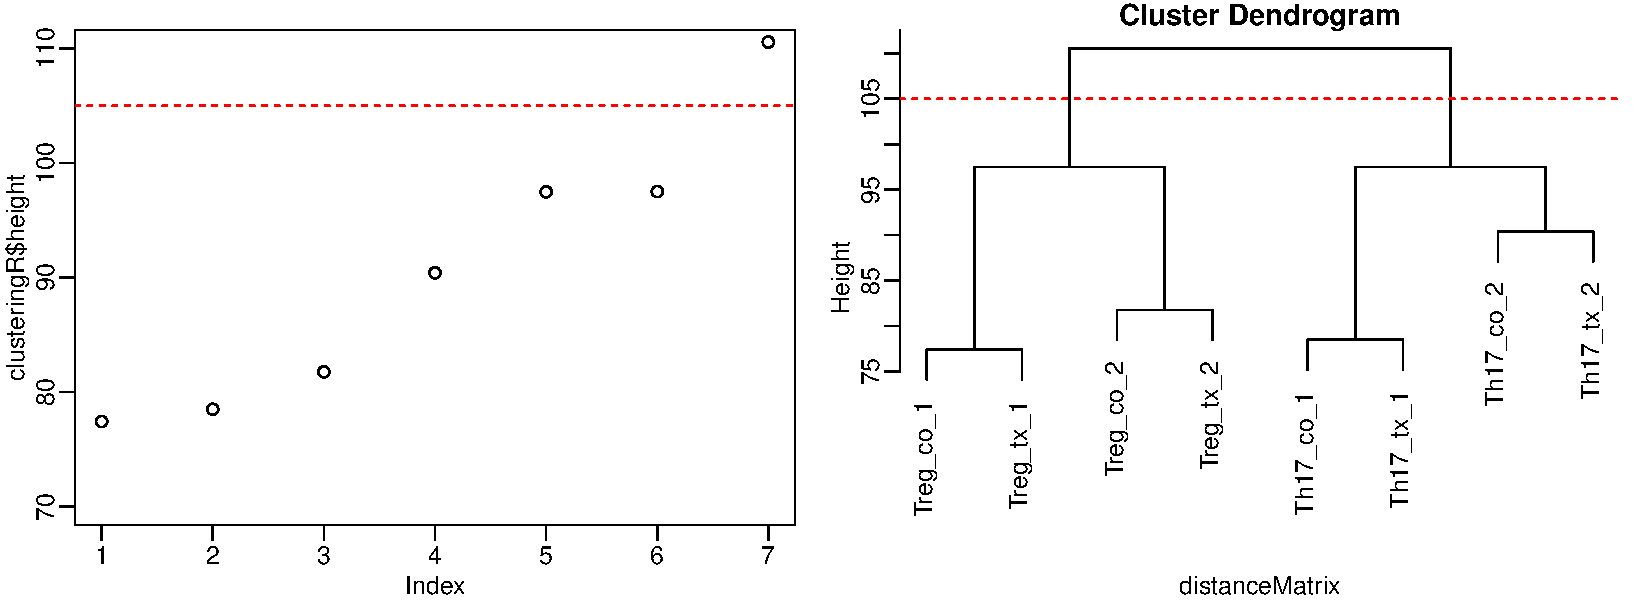
\includegraphics{Osorio_Daniel_E1-003}
\item How many clusters would you say there are, and why? \textit{From the height plot, there are two main clusters given by the high separation between the last point and the others. However, from the cluster plot is evident that inside these two there are other two subclusters.}
\item How would you explain the apparent clustering? \textit{Main clusters are formed by cell type (Th17 and Treg) and the clusters inside are driven by the donor.}
\end{enumerate}
\item Carry out principal component analysis to explore structure among the arrays (columns)
\begin{Schunk}
\begin{Sinput}
> PC <- prcomp(t(data))
\end{Sinput}
\end{Schunk}
\begin{enumerate}
\item Should you standardize or not? Does it matter in this case? In what follows, so we all match answers, do not standardize the columns. \textit{As all the columns seem to have approximately the same variability, it's not required to standardize the columns. See below:}
\begin{Schunk}
\begin{Sinput}
> apply(data,2,var)
\end{Sinput}
\begin{Soutput}
Th17_co_1 Th17_tx_1 Treg_co_1 Treg_tx_1  
 3.939703  3.926221  3.903509  3.944170  
 
Th17_co_2 Th17_tx_2 Treg_co_2 Treg_tx_2
 3.823271  3.933689  3.959382  3.884836 
\end{Soutput}
\end{Schunk}

\item What is the proportion of total variance explained by the first principal component? By the second principal component?
\begin{Schunk}
\begin{Sinput}
> summary(PC)$importance[,1:2]
\end{Sinput}
\begin{Soutput}
                            PC1      PC2
Standard deviation     36.74840 29.73041
Proportion of Variance  0.28287  0.18515
Cumulative Proportion   0.28287  0.46802
\end{Soutput}
\end{Schunk}
\item What are the coefficients that define the first principal component’s linear combination of the columns (in other words, what is the first eigenvector of the $8 \times 8$ sample covariance matrix)? Comment. What do these tell you, if anything, about the data? \textit{The coefficients of this eigenvector split the samples by cell types in the same way as the cluster analysis. All the Th17 have negative values meanwhile all Treg have positive ones.}
\begin{Schunk}
\begin{Sinput}
> PC$x[,1]
\end{Sinput}
\begin{Soutput}
Th17_co_1 Th17_tx_1 Treg_co_1 Treg_tx_1 
-32.46593 -32.64027  36.92041  39.17638 

Th17_co_2 Th17_tx_2 Treg_co_2 Treg_tx_2 
-38.71109 -32.78506  26.25808  34.24749 
\end{Soutput}
\end{Schunk}
\item Provide a scatterplot of the first two principal components. Comment. Are there any inter- esting patterns, clustering, outliers? If so, how would you explain them? \textit{As well as in cluster analysis there are two main clusters in the PC1 driven by the cell type and other two in the PC2 driven by the donor.}
\begin{Schunk}
\begin{Sinput}
> par(mar=c(2.5,2.5,1,1), mgp = c(1.5,0.5,0))
> plot(PC$x[,1:2])
\end{Sinput}
\end{Schunk}
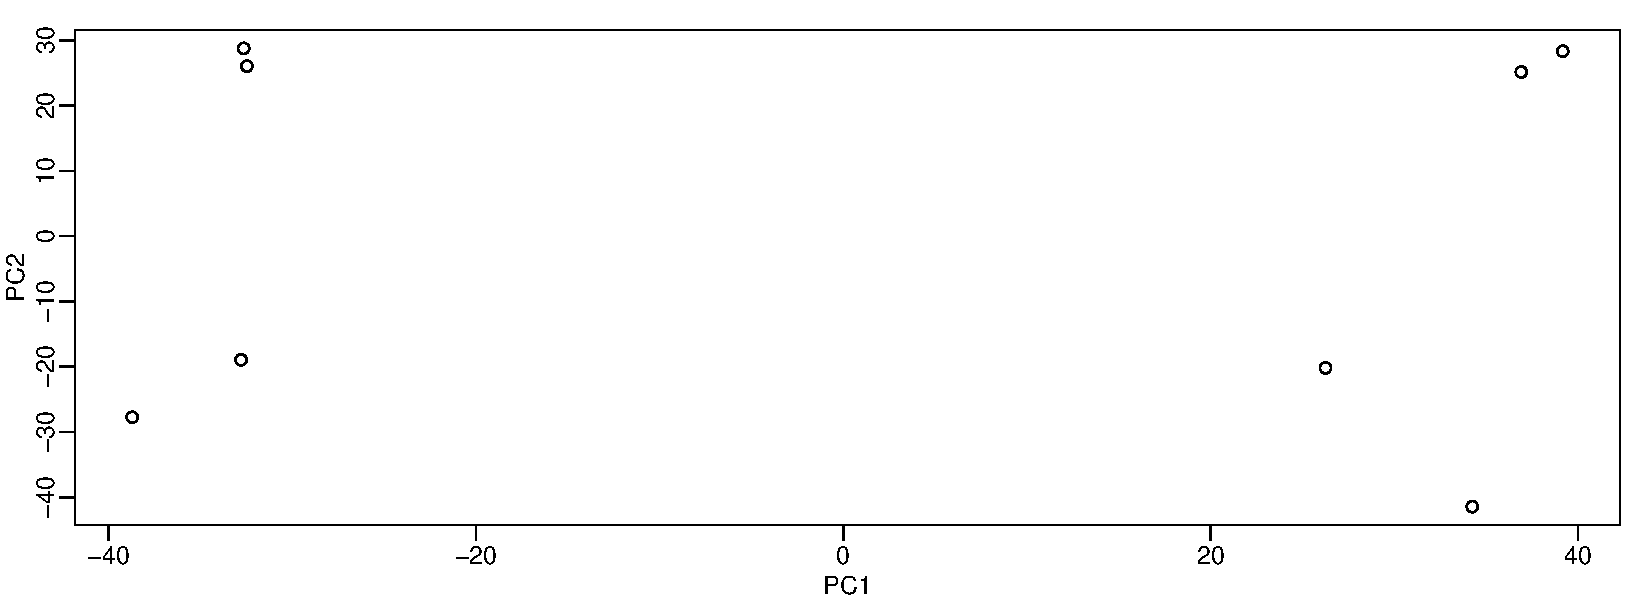
\includegraphics{Osorio_Daniel_E1-008}
\end{enumerate}
\item Use two-sample t-tests (assuming unequal variances, the default in R) to test for diffrential expression between the 4 treatment and 4 control arrays
\begin{Schunk}
\begin{Sinput}
> isControl <- grepl("co", colnames(data))
> diffM <- data[,isControl] - data[,!isControl]
> pValues  <- apply(diffM, 1, function(X){
+   t.test(X)$p.value
+ })
\end{Sinput}
\end{Schunk}
\begin{enumerate}
\item Report a histogram of the p-values. Comment on its shape (does it look as you would expect, are there any worrisome features, do there appear to be many genes for which mean expression differs between control and treatment conditions). \textit{Distribution is uniform. There appear to be less differentially expressed genes than the expected by chance. }
\begin{Schunk}
\begin{Sinput}
> par(mar=c(2.5,2.5,1,1), mgp = c(1.5,0.5,0))
> hist(pValues, probability = TRUE)
> abline(v = 0.05, col = "red", lty = 2)
\end{Sinput}
\end{Schunk}
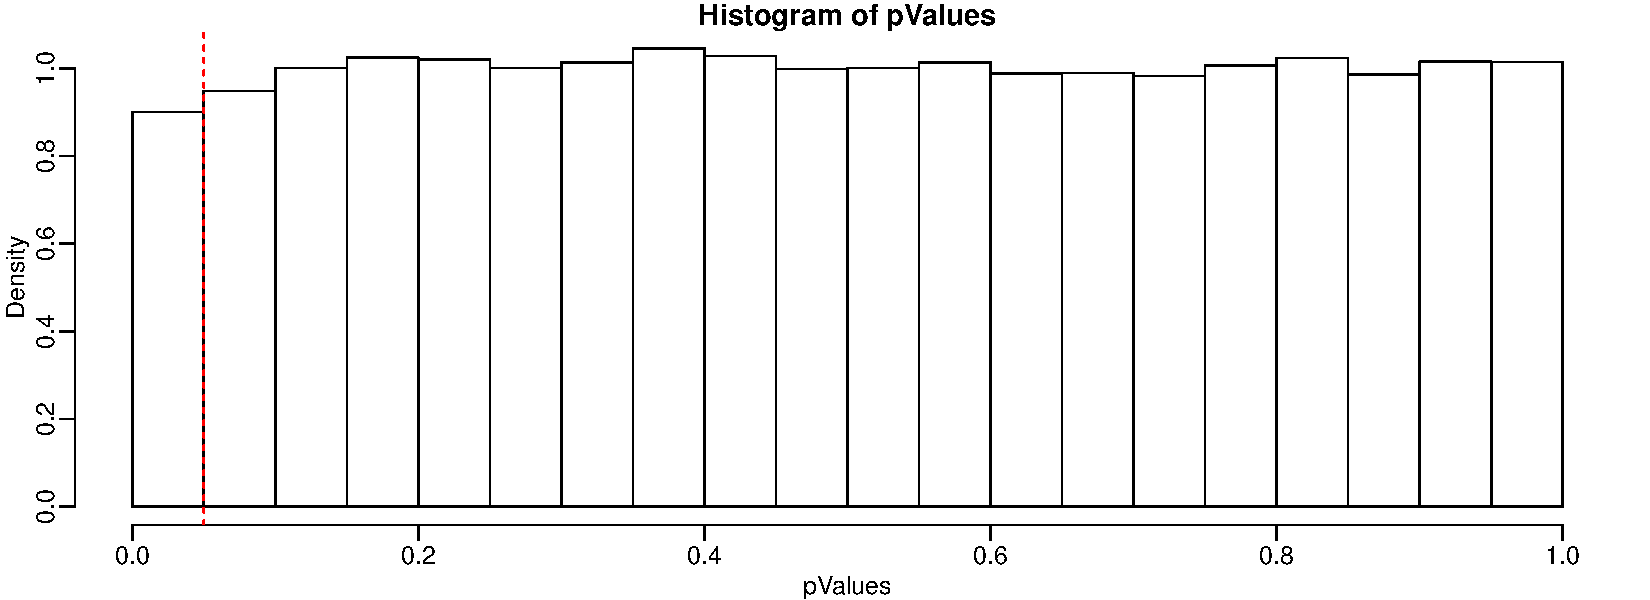
\includegraphics{Osorio_Daniel_E1-010}
\item If none of the genes were differentially expressed, what proportion of the p-values would you expect to be <0.05? \textit{Approximately 5\%} What proportion of p-values are <0.05? \textit{Around 4.5\%} What does this tell you about whether there are many genes for which mean expression differs between control and treatment conditions? \textit{There is not enough evidence supporting a difference between treatment and control samples.}
\begin{Schunk}
\begin{Sinput}
> mean(pValues < 0.05)
\end{Sinput}
\begin{Soutput}
[1] 0.04500438
\end{Soutput}
\end{Schunk}
\item Convert the p-values to q-values using p.adjust (use method = “fdr”). How many genes do you call differentially expressed at an estimated FDR of 0.05? \textit{None}
\begin{Schunk}
\begin{Sinput}
> table(p.adjust(pValues) < 0.05)
\end{Sinput}
\begin{Soutput}
FALSE 
53617 
\end{Soutput}
\end{Schunk}
\end{enumerate}
\item The MAX gene is present in multiple species. The versions of the gene in human, mouse are said to be homologous
\begin{Schunk}
\begin{Sinput}
> library(seqinr)
> choosebank("genbank")
\end{Sinput}
\end{Schunk}
\begin{enumerate}
\item Consider the global alignment of the sequences of this gene in human (Homo sapiens) and mouse (Mus musculus). Use seqinr to download the DNA sequences. You will get multiple sequences for each species. Use third sequence (BC004516.MAX) for human and first sequence (BC138671.MAX) for mouse to answer the following questions. The lengths of the human and mouse sequences will be the same.
\begin{Schunk}
\begin{Sinput}
> hsaMAX <- query(listname="MAX", query="SP=Homo sapiens AND K=MAX")
> hsaMAX <- getSequence(hsaMAX$req[[3]])
> mmusMAX <- query(listname="MAX", query="SP=Mus musculus AND K=MAX")
> mmusMAX <- getSequence(mmusMAX$req[[1]])
\end{Sinput}
\end{Schunk}
\begin{enumerate}
\item Comparing the human and mouse versions of MAX, what proportion of bases dffer? \textit{Approximately 4\%}
\begin{Schunk}
\begin{Sinput}
> mean(hsaMAX != mmusMAX)
\end{Sinput}
\begin{Soutput}
[1] 0.03933747
\end{Soutput}
\end{Schunk}
\item Compare the human and mouse versions of MAX with respect to GC content of the bases? \textit{Their proportions of GC contents are almost identical around the 50\%}
\begin{Schunk}
\begin{Sinput}
> sum(table(hsaMAX)[c("g","c")])/length(hsaMAX)
\end{Sinput}
\begin{Soutput}
[1] 0.5403727
\end{Soutput}
\begin{Sinput}
> sum(table(mmusMAX)[c("c","g")])/length(mmusMAX)
\end{Sinput}
\begin{Soutput}
[1] 0.5341615
\end{Soutput}
\end{Schunk}
\end{enumerate}
\item Consider the global alignment of these two DNA sequences: GAG and GTAG. Let the score for a match be +1, the score for a mismatch be -1, and the score for a gap be -2 . Write down the score matrix for this alignment, and fill in all of the cells. (Note: you do not have to find me any alignment just fill out the score matrix i.e each cell value with direction.)
\begin{center}
\begin{tabular}{|p{0.5cm}|p{0.5cm}|p{0.5cm}|p{0.5cm}|p{0.5cm}|p{0.5cm}|}
\hline
&&&&&\\[10pt]
\hline
&&&&& \\[10pt]
\hline
&&&&& \\[10pt]
\hline
&&&&& \\[10pt]
\hline
&&&&& \\[10pt]
\hline
\end{tabular}
\end{center}
\end{enumerate}
\end{enumerate}
\end{enumerate}
\end{document}
